\chapter{KHẢO SÁT VÀ PHÂN TÍCH YÊU CẦU}
Dựa trên phạm vi hiện tại của đề tài, chương 2 tập trung khảo sát nhu cầu chấm phiếu trắc nghiệm OMR bằng ảnh chụp và phân tích các yêu cầu tương ứng với hệ thống đã triển khai. Hệ thống hiện là một ứng dụng web OMR: giáo viên đăng ký/đăng nhập, tạo bài thi, cấu hình nhiều mã đề, chấm một hoặc nhiều ảnh phiếu, xem lịch sử kết quả và xuất báo cáo. Luồng nhận diện sử dụng xử lý ảnh có tính xác định bằng OpenCV~\cite{opencv}/NumPy, Form Profile, ROI và marker định vị.

\section{Khảo sát hiện trạng}
Qua khảo sát thực tế tại một số trường trung học và đại học, quá trình chấm điểm phiếu trắc nghiệm thường được thực hiện theo ba hình thức chính:

\begin{itemize}
    \item \textbf{Chấm thủ công hoàn toàn}: Giáo viên đối chiếu từng câu với đáp án mẫu trên giấy. Cách làm này dễ triển khai nhưng tốn nhiều thời gian, đặc biệt khi số lượng phiếu lớn hoặc bài thi có nhiều mã đề.
    \item \textbf{Dùng máy quét OMR chuyên dụng}: Một số cơ sở giáo dục có điều kiện đầu tư máy quét và phần mềm OMR. Phương án này cho tốc độ cao nhưng chi phí thiết bị, bảo trì và vận hành chưa phù hợp với nhiều trường học quy mô nhỏ.
    \item \textbf{Dùng ứng dụng chấm phiếu của bên thứ ba}: Một số ứng dụng di động hỗ trợ chụp ảnh và chấm phiếu, nhưng thường bị giới hạn số lượt chấm, phụ thuộc mẫu phiếu cố định hoặc khó tích hợp dữ liệu với hệ thống quản lý nội bộ.
\end{itemize}

Bên cạnh đó, các giáo viên cũng phản ánh một số hạn chế chung của các phương pháp hiện tại:

\begin{itemize}
    \item Chi phí đầu tư cho thiết bị và phần mềm bản quyền còn cao so với nhu cầu chấm bài định kỳ trong lớp học.
    \item Việc quản lý nhiều mã đề trong cùng một bài thi dễ nhầm lẫn nếu phải tách phiếu và nhập điểm thủ công.
    \item Ảnh chụp bằng điện thoại thường có góc nghiêng, bóng đổ hoặc ánh sáng không đều, nên hệ thống cần có bước chuẩn hóa phối cảnh, ROI và kiểm tra marker.
    \item Giáo viên cần xem lại ảnh overlay, lịch sử từng lượt chấm và xuất Excel/PDF thay vì chỉ nhận một điểm số đơn lẻ.
\end{itemize}

\section{Tổng quan chức năng}
\begin{figure}[H]
    \centering
    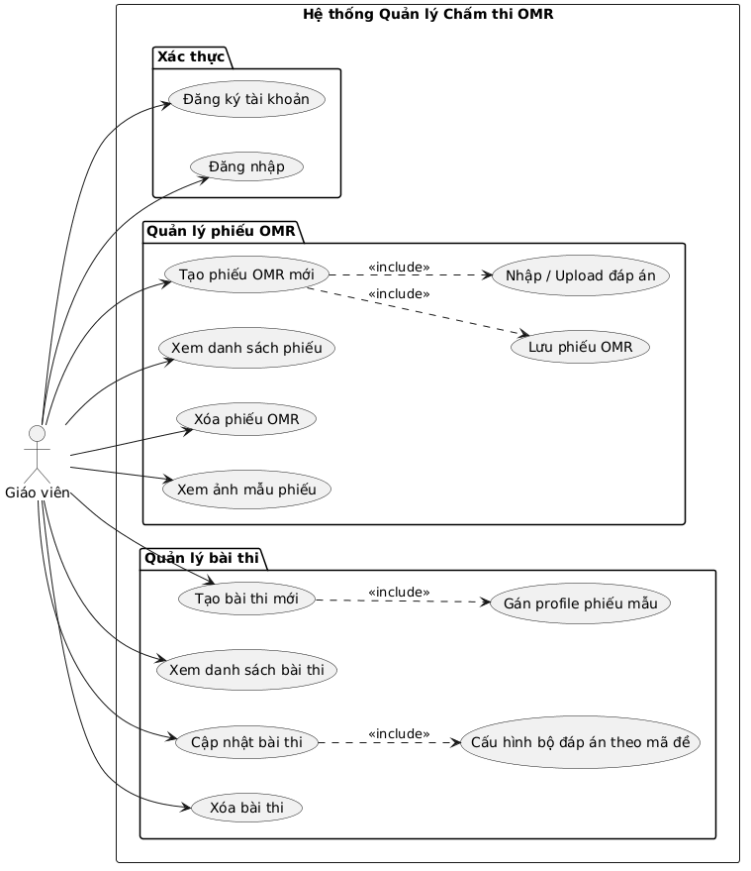
\includegraphics[
        width=\linewidth,
        height=0.85\textheight,
        keepaspectratio
    ]{figures/overview.jpg}
    \caption{Biểu đồ use case tổng quan}
    \label{fig:usecase_overview}
\end{figure}

Biểu đồ use case tổng quan mô tả các tương tác chính giữa giáo viên và Hệ thống Quản lý Chấm thi OMR. Đối tượng sử dụng chính là giáo viên; các thao tác sau đăng nhập được gắn với \texttt{uid} để phân tách dữ liệu theo người dùng. Các chức năng hiện tại được chia thành bốn nhóm nghiệp vụ cốt lõi như sau:

\begin{itemize}
    \item \textbf{Nhóm Xác thực (Authentication)}: Cung cấp đăng ký, đăng nhập thường và đăng nhập Google. Frontend lưu thông tin người dùng trong \path{localStorage}; backend kiểm tra \texttt{uid} ở các endpoint nghiệp vụ để đảm bảo thao tác gắn với tài khoản hợp lệ.
    \item \textbf{Nhóm Mẫu phiếu và Form Profile}: Mỗi Form Profile là một file cấu hình JSON lưu toàn bộ tham số OCR/OMR cho một loại phiếu trắc nghiệm cụ thể, bao gồm số câu, số lựa chọn, số chữ số mã số sinh viên, tọa độ bốn góc, vùng xác định mã sinh viên/mã đề/câu trả lời/họ tên. Giáo viên xem danh sách profile cùng ảnh/PDF mẫu phiếu tương ứng để xác định loại phiếu phù hợp, rồi gắn profile đó vào bài thi khi tạo -- đây là điều kiện bắt buộc vì profile quyết định cách hệ thống nhận diện và giải mã từng vùng trên phiếu. 
    \item \textbf{Nhóm Quản lý bài thi và đáp án}: Giáo viên tạo, cập nhật, xóa bài thi, cấu hình nhiều bộ đáp án theo mã đề ba chữ số. Cách tổ chức này phù hợp với thực tế trộn đề, vì một bài thi có thể chứa nhiều mã đề và hệ thống tự chọn bộ đáp án dựa trên mã đề đọc được trên phiếu.
    \item \textbf{Nhóm Chấm điểm và kết quả}: Giáo viên chấm một ảnh hoặc chấm hàng loạt tối đa 50 ảnh, dùng Smart Camera Scanner hoặc upload ảnh từ thiết bị, xem thống kê/lịch sử, xem chi tiết bản ghi, ảnh overlay và xuất Excel/PDF.
\end{itemize}

\subsection{Quy trình nghiệp vụ chấm bài}
\begin{figure}[H]
  \centering
  \includegraphics[height=0.78\textheight, keepaspectratio]{figures/Tongquan.jpg}
  \caption{Quy trình nghiệp vụ chấm bài}
  \label{fig:Tongquan}
\end{figure}

Quy trình nghiệp vụ chấm bài được chia thành bốn giai đoạn chính, nối tiếp nhau từ khi giáo viên đăng nhập cho đến khi nhận kết quả và xuất báo cáo.

\textbf{Giai đoạn 1 -- Chuẩn bị bài thi (UC-01 đến UC-05)} \textit{(phía Giáo viên)}\textbf{.}
Giáo viên đăng nhập hoặc đăng ký tài khoản (UC-01, UC-02). Sau đó, giáo viên có thể xem danh sách Form Profile và ảnh mẫu phiếu (UC-03) để chọn loại phiếu phù hợp, rồi tạo hoặc chỉnh sửa bài thi gắn với profile đó (UC-04). Vì một đề thi thường có nhiều mã đề khác nhau, giáo viên nhập bộ đáp án riêng cho từng mã đề vào trường \path{answer_sets} (UC-05). Dữ liệu này được lưu dưới dạng JSON ánh xạ mã đề ba chữ số tới danh sách chỉ số đáp án theo thứ tự câu hỏi (A=0, B=1, C=2, D=3), ví dụ \texttt{"001"} $\to$ \texttt{[0,2,1,3,\ldots]} nghĩa là câu~1 chọn A, câu~2 chọn C, câu~3 chọn B. Đây là điều kiện bắt buộc trước khi chấm; nếu bài thi chưa có đáp án, backend từ chối request và trả thông báo lỗi \textit{``Kho đáp án của bài thi đang trống''}.

\textbf{Giai đoạn 2 -- Thu nhận ảnh (UC-06, UC-07)} \textit{(phía Giáo viên)}\textbf{.}
Giáo viên có hai cách cung cấp ảnh phiếu cho hệ thống. Cách thứ nhất là dùng \textit{Smart Camera Scanner} (UC-06): tính năng này sử dụng \texttt{WebRTC MediaDevices API}~\cite{webrtc} để lấy luồng video camera trực tiếp trên trình duyệt. Frontend phân tích từng frame mỗi khoảng 130ms, tính tỷ lệ pixel tối tại bốn vùng marker góc phiếu và kiểm tra độ sáng trung tâm; khi phiếu đủ điều kiện (phát hiện được bốn marker, độ sáng đạt ngưỡng), hệ thống tự động chụp và lưu frame vào danh sách ảnh mà không cần giáo viên nhấn nút chụp. Cách thứ hai là \textit{upload ảnh thủ công} (UC-07): giáo viên chọn một hoặc nhiều file ảnh từ thư viện thiết bị và chúng được thêm vào cùng danh sách ảnh. Sau khi tích lũy đủ ảnh cần chấm, giáo viên nhấn nút \textbf{Chấm bài} để chuyển sang giai đoạn xử lý.

\textbf{Giai đoạn 3 -- Xử lý và chấm điểm (UC-08, UC-09)} \textit{(phía Hệ thống)}\textbf{.}
Khi giáo viên nhấn nút Chấm bài, frontend kiểm tra số lượng ảnh đã thu nhận: nếu \path{pickedFiles.length > 1}, frontend gọi \path{POST /api/omr/grade-batch} (tối đa 50 ảnh -- UC-09); ngược lại gọi \path{POST /api/omr/grade} cho ảnh đơn (UC-08). Router trong \path{grading.py} kiểm tra định danh người dùng (\texttt{uid}), đọc thông tin bài thi và Form Profile, sau đó gọi hàm \texttt{process\_omr\_exam()} trong \path{omr_service.py}. Pipeline 15 bước thực hiện tuần tự: chuẩn hóa phối cảnh về kích thước 1000$\times$1400 pixel, nhị phân hóa thích nghi, phát hiện marker định vị, dựng các vùng ROI, giải mã mã số sinh viên, giải mã mã đề và giải mã đáp án. Nếu số câu không chắc chắn đạt ngưỡng kích hoạt $\max(4,\ \lceil 0{,}60 \times Q \rceil)$ câu, cơ chế \textbf{MCQ Map Search Rescue} tự động thử 54 biến thể hình học của lưới câu hỏi (6 hệ số line-scale $\times$ 9 bước dịch chuyển) để tìm cấu hình cho kết quả ổn định hơn. Sau khi có kết quả decode, hệ thống tra \path{answer_sets} theo mã đề vừa đọc từ phiếu và tính điểm từng câu.

\textbf{Giai đoạn 4 -- Lưu kết quả và phản hồi (UC-10 đến UC-13)} \textit{(Hệ thống và Giáo viên)}\textbf{.}
Kết quả chấm được lưu vào bảng \path{omr_grade_result} với đầy đủ điểm, mã sinh viên, mã đề, đường dẫn ảnh overlay, ảnh cắt kết quả trả lời (UC-10). Trường \path{last_result} trên \path{omr_assignment} đồng thời được cập nhật để giao diện danh sách bài thi hiển thị thông tin lượt chấm gần nhất. Backend trả JSON kèm URL ảnh overlay màu để giáo viên kiểm tra trực quan. Giáo viên có thể xem thống kê và lọc lịch sử chấm (UC-11), xem chi tiết từng bản ghi cùng ảnh overlay (UC-12) và xuất toàn bộ kết quả ra file Excel hoặc PDF (UC-13).

Quy trình có ba nhánh xử lý ngoại lệ quan trọng:\\
(i) nếu ảnh không đọc được hoặc không phát hiện được phiếu, backend trả lỗi HTTP 400 mà không lưu bản ghi lịch sử. \\
(ii) nếu mã đề đọc từ phiếu không tìm thấy trong \path{answer_sets}, hệ thống dùng bộ đáp án đang được đặt làm active làm fallback và ghi cảnh báo vào kết quả.\\ 
(iii) trong chấm lô batch, mỗi ảnh lỗi chỉ ghi \texttt{success: false} vào phần tử tương ứng trong mảng kết quả mà không dừng toàn bộ lô. 

\subsection{Phân rã use case mức chi tiết}
Bảng~\ref{tab:phan-ra-usecase-chi-tiet} trình bày phân rã chi tiết các use case chính trong hệ thống. Mỗi use case được mô tả theo mã định danh, nhóm chức năng mức cao, use case con, module triển khai, dữ liệu đầu vào chính và kết quả đầu ra tương ứng.

\scriptsize
\setlength{\tabcolsep}{3pt}
\renewcommand{\arraystretch}{1.25}

\begin{longtable}{|
>{\RaggedRight\arraybackslash}p{0.9cm}|
>{\RaggedRight\arraybackslash}p{1.8cm}|
>{\RaggedRight\arraybackslash}p{2.3cm}|
>{\RaggedRight\arraybackslash}p{2.7cm}|
>{\RaggedRight\arraybackslash}p{2.2cm}|
>{\RaggedRight\arraybackslash}p{3.0cm}|}
\caption{Phân rã use case mức chi tiết}
\label{tab:phan-ra-usecase-chi-tiet} \\

\hline
\textbf{Mã UC} &
\textbf{Use case mức cao} &
\textbf{Use case con} &
\textbf{Module triển khai} &
\textbf{Dữ liệu chính} &
\textbf{Kết quả} \\
\hline
\endfirsthead

\hline
\textbf{Mã UC} &
\textbf{Use case mức cao} &
\textbf{Use case con} &
\textbf{Module triển khai} &
\textbf{Dữ liệu chính} &
\textbf{Kết quả} \\
\hline
\endhead

UC-01 & Xác thực & Đăng nhập & \path{auth.py}, \path{LoginPage.tsx} & email, password & Lưu thông tin user vào \path{localStorage} \\
\hline
UC-02 & Xác thực & Đăng ký & \path{auth.py}, \path{RegisterPage.tsx} & \path{user_name}, email, phone, password & Bản ghi mới trong \path{users} \\
\hline
UC-03 & Mẫu phiếu & Xem danh sách Form Profile (loại phiếu hỗ trợ) và ảnh/PDF mẫu để chọn khi tạo bài thi & \path{profiles.py}, \path{templates.py}, \path{MultichoicePage.tsx} & profile JSON, sample file & Danh sách profile và ảnh/PDF mẫu \\
\hline
UC-04 & Quản lý bài thi & Tạo/sửa/xóa bài thi & \path{assignments.py} & uid, aid, title, profile code & Bản ghi \path{omr_assignment} \\
\hline
UC-05 & Quản lý đáp án & Cấu hình nhiều mã đề & \path{answer_sets}, \path{MultichoicePage.tsx} & code, answers & JSON \path{answer_sets} theo mã đề \\
\hline
UC-06 & Chụp ảnh & Smart Camera Scanner & \path{MultichoicePage.tsx}, \path{evaluateAlignment()} & video frame, scanner hint & Ảnh JPEG tự chụp khi đủ marker \\
\hline
UC-07 & Chụp ảnh & Upload ảnh đơn/lô & \path{MultichoicePage.tsx} & File ảnh & FormData gửi backend \\
\hline
UC-08 & Chấm điểm & Chấm 1 phiếu & \path{grading.py}, \path{omr_service.py} & image, uid, aid, profile & JSON điểm, MSSV, mã đề và ảnh overlay \\
\hline
UC-09 & Chấm điểm & Chấm hàng loạt & \path{grading.py}, \path{omr_service.py} & tối đa 50 ảnh & Danh sách kết quả và zip overlay \\
\hline
UC-10 & Kết quả & Lưu lịch sử & \path{grading.py}, \path{grade_results.py}, \path{assignments.py} & GradeRecord, OMRGradeResult & Thêm bản ghi \path{omr_grade_result}, cập nhật \path{last_result}, \path{graded_count} \\
\hline
UC-11 & Kết quả & Xem/lọc thống kê & \path{StatsPanel.tsx} & records, keyword & Danh sách bản ghi phù hợp \\
\hline
UC-12 & Kết quả & Xem chi tiết bản ghi & route \path{/multichoice/record-detail/:testId/:recordId} & recordId & Chi tiết ảnh overlay và câu trả lời \\
\hline
UC-13 & Kết quả & Xuất Excel/PDF & \path{ExportPanel.tsx} & records & File \path{.xlsx} hoặc \path{.pdf} \\
\hline
\end{longtable}

\normalsize
\setlength{\tabcolsep}{4pt}
\renewcommand{\arraystretch}{1.18}

\section{Yêu cầu phi chức năng}
\subsection{Tính bảo mật}
Hệ thống được thiết kế theo nguyên tắc xác thực tại tầng API, kiểm soát truy cập theo người dùng và hạn chế tối đa các vector tấn công phổ biến.

\begin{itemize}[leftmargin=1.5cm]
  \item \textbf{Xác thực người dùng}: Mọi thao tác quản lý dữ liệu như tạo bài thi, cập nhật đáp án, chấm bài và xem lịch sử đều yêu cầu \texttt{uid} hợp lệ trong request. Hệ thống kiểm tra \texttt{uid} tại từng endpoint thông qua hàm \texttt{\_validate\_uid()}, từ chối yêu cầu nếu tham số không hợp lệ hoặc không tồn tại trong cơ sở dữ liệu.
  \item \textbf{Phân quyền theo sở hữu}: Mỗi bài thi (\texttt{OMRAssignment}), template/profile OMR (\texttt{OMRTest}) và bản ghi kết quả (\texttt{OMRGradeResult}) đều được gắn với \texttt{uuid} của giáo viên. Các truy vấn cơ sở dữ liệu lọc theo \texttt{uid} và \texttt{aid}/\texttt{omrid}/\texttt{recordId} tương ứng, hạn chế người dùng truy cập dữ liệu của nhau.
  \item \textbf{Kiểm soát CORS}: Backend cấu hình CORS chỉ cho phép các nguồn gốc từ \texttt{localhost}, \texttt{127.0.0.1} và dải địa chỉ LAN nội bộ (\texttt{192.168.x.x}), hạn chế các yêu cầu cross-origin từ domain lạ.
  \item \textbf{Làm sạch dữ liệu đầu vào}: Tên file upload được lọc qua \texttt{os.path.basename()} trước khi ghi xuống đĩa, ngăn chặn tấn công path traversal. Mã đề thi (\texttt{omr\_code}) bắt buộc đúng định dạng 3 chữ số bằng regex \texttt{\textbackslash d\{3\}}; mã profile được chuẩn hóa về ký tự an toàn trước khi dùng làm tên file JSON.
  \item \textbf{Giới hạn prototype}: Phiên bản hiện tại lưu mật khẩu dạng plain-text, frontend lưu user trong \path{localStorage} và chưa có \texttt{ProtectedRoute}/JWT production. Khi triển khai thật, cần băm mật khẩu bằng bcrypt/argon2, dùng JWT hoặc session có thời hạn và cấu hình secret qua biến môi trường.
\end{itemize}

\subsection{Khả năng lưu trữ}
Hệ thống áp dụng chiến lược lưu trữ phân tán giữa cơ sở dữ liệu quan hệ và hệ thống file để cân bằng hiệu năng và dung lượng.

\begin{itemize}[leftmargin=1.5cm]
  \item \textbf{Cơ sở dữ liệu quan hệ}: PostgreSQL lưu trữ metadata nghiệp vụ gồm thông tin người dùng, bài thi, template OMR, cấu hình template và kết quả chấm. Dữ liệu bán cấu trúc như \path{answer_sets}, \path{last_result}, \texttt{omr\_answer}, \path{info_fields} và \path{result_json} được lưu dưới dạng JSON.
  \item \textbf{Khởi tạo bằng Docker}: Với môi trường local/demo, PostgreSQL được chạy như một service riêng trong Docker Compose~\cite{docker} (\texttt{postgres:16-alpine}) và lưu dữ liệu bằng named volume \texttt{pgdata}. Backend đợi database healthy trước khi khởi động và tự tạo bảng bằng SQLAlchemy khi database rỗng.
  \item \textbf{Bảng lịch sử chấm độc lập}: Ngoài \path{last_result} trên \path{omr_assignment} để tương thích giao diện cũ, hệ thống đã bổ sung bảng \path{omr_grade_result} để lưu từng lượt chấm với \texttt{aid}, \texttt{uuid}, \texttt{omrid}, MSSV, mã đề, điểm, đường dẫn ảnh kết quả/crop và JSON kết quả đầy đủ.
  \item \textbf{Lưu trữ file}: Ảnh phiếu thi gốc, ảnh kết quả có overlay màu, ảnh crop vùng MSSV/MCQ/họ tên, file JSON confidence của từng bong bóng, file ZIP kết quả batch và ảnh/PDF template được lưu trong \texttt{storage/uploads} (\texttt{omr}, \texttt{omr\_templates}, \texttt{omr\_data}). Khi chạy Docker, thư mục \path{./storage} được mount vào container backend để dữ liệu runtime không mất khi recreate container. Static file server tích hợp trong FastAPI phục vụ các file này qua đường dẫn \path{/static/}.
  \item \textbf{Metadata template trong SQL}: Các trường metadata của template như \path{template_image}, \path{info_fields}, \path{options}, \path{rows_per_block} và \path{student_id_digits} được lưu trong bảng \path{omr_test}.
  \item \textbf{File đáp án tạm}: Backend vẫn có thư mục \path{storage/uploads/answer_keys/omr} để hỗ trợ parse file đáp án Word/PDF/TXT ở các API tương thích. Với giao diện chính hiện tại, giáo viên cấu hình đáp án trực tiếp theo từng mã đề trong \path{answer_sets}; nếu có file upload tạm, sau khi parse dữ liệu được lưu vào SQL và file được xóa để giảm dữ liệu rác.
  \item \textbf{Dung lượng ước tính}: Mỗi phiếu thi sau xử lý sinh ra khoảng 2--5 MB file ảnh kết quả. Với quy mô 1.000 bài chấm mỗi kỳ thi, hệ thống cần dự phòng khoảng 5--10 GB dung lượng lưu trữ cho mỗi năm học. Kết quả chấm hàng loạt được đóng gói ZIP để giảm số lần truyền tải.
\end{itemize}

\subsection{Tính dễ dùng}
Hệ thống được thiết kế hướng đến giáo viên không có chuyên môn kỹ thuật, ưu tiên quy trình thao tác tối giản và phản hồi trực quan.

\begin{itemize}[leftmargin=1.5cm]
  \item \textbf{Giao diện một trang (SPA)}: Toàn bộ luồng chấm điểm từ chọn bài thi, tải ảnh lên đến xem kết quả diễn ra trên một màn hình duy nhất mà không cần tải lại trang, giảm thiểu thao tác điều hướng.
  \item \textbf{Smart Camera Scanner}: Tính năng quét camera tích hợp tự động nhận diện bốn góc phiếu thi theo thời gian thực, khóa khung hình khi điều kiện ánh sáng và góc chụp đạt yêu cầu và tự động chụp mà không cần người dùng nhấn nút. Điều này đặc biệt hữu ích khi chấm số lượng lớn tại lớp học.
  \item \textbf{Phản hồi lỗi rõ ràng}: API trả về thông báo lỗi bằng tiếng Việt có nội dung cụ thể, ví dụ ``Đề thi này chưa được cung cấp đáp án'', giúp giáo viên tự xử lý mà không cần hỗ trợ kỹ thuật.
  \item \textbf{Quản lý đáp án theo mã đề}: Giao diện chính hiện cho giáo viên cấu hình đáp án trực tiếp bằng các lựa chọn A/B/C/D theo từng mã đề.
  \item \textbf{Xuất kết quả}: Danh sách kết quả có thể xuất ra file Excel (\texttt{.xlsx}) hoặc PDF ngay trên trình duyệt, phục vụ nhu cầu lưu trữ và báo cáo mà không cần phần mềm bổ sung.
\end{itemize}

\subsection{Khả năng mở rộng}
Kiến trúc hệ thống được thiết kế theo hướng module hóa, cho phép bổ sung tính năng và tăng quy mô mà không cần tái cấu trúc toàn bộ.

\begin{itemize}[leftmargin=1.5cm]
  \item \textbf{Tách biệt frontend và backend}: React SPA giao tiếp với FastAPI hoàn toàn qua REST API. Trong Docker, frontend được build thành file tĩnh và phục vụ bằng Caddy; Caddy reverse proxy các đường dẫn \path{/api/*} và \path{/static/*} về backend. Hai tầng có thể triển khai độc lập, cho phép mở rộng backend theo chiều ngang hoặc thay thế frontend mà không ảnh hưởng đến logic nghiệp vụ.
  \item \textbf{Form Profile linh hoạt}: Cấu hình nhận diện phiếu thi được lưu dưới dạng file JSON độc lập trong \path{storage/uploads/omr_data/profiles}. Để hỗ trợ loại phiếu mới, chỉ cần thêm file mẫu và cấu hình profile tương ứng; metadata nghiệp vụ của template được đồng bộ vào SQL để dễ quản lý.
  \item \textbf{Pipeline xử lý ảnh có tham số hóa}: Toàn bộ các tham số xử lý ảnh như ngưỡng nhị phân, tỉ lệ vùng bong bóng, chiến lược ROI và bộ giải mã MCQ đều có thể ghi đè qua profile mà không cần sửa code nguồn, cho phép tinh chỉnh độ chính xác theo từng loại phiếu mà không ảnh hưởng đến các loại phiếu khác.
  \item \textbf{Hỗ trợ đa mã đề}: Cấu trúc \path{answer_sets} lưu danh sách bộ đáp án theo mã đề, ví dụ mã 001, 002, 003, cho phép một bài thi quản lý nhiều đề thi khác nhau. Hệ thống tự động chọn đáp án phù hợp dựa trên mã đề nhận diện từ phiếu.
  \item \textbf{Cơ chế MCQ Map Search Rescue}: Tính năng tự động hiệu chỉnh lưới MCQ được triển khai trong \path{omr_service.py}, có thể bật/tắt qua cấu hình profile \path{disable_mcq_rescue}. Cơ chế này thử các biến thể line-height/top-shift khi số câu không chắc chắn vượt ngưỡng.
  \item \textbf{Sẵn sàng tách object storage}: Các file nhị phân lớn được tham chiếu bằng đường dẫn thay vì lưu trực tiếp vào SQL. Khi triển khai lên AWS, lớp lưu trữ này có thể chuyển từ filesystem cục bộ sang S3 mà không thay đổi mô hình dữ liệu chính.
  \item \textbf{Tùy chọn database ngoài}: Docker Compose cung cấp PostgreSQL để khởi tạo nhanh, nhưng production có thể dùng PostgreSQL bên ngoài/RDS bằng cách ghi đè \texttt{DATABASE\_URL} và bỏ phụ thuộc \texttt{db} trong compose override.
\end{itemize}

\subsection{Hiệu năng}
Hệ thống áp dụng nhiều kỹ thuật tối ưu để đảm bảo thời gian phản hồi chấp nhận được trong điều kiện tài nguyên phần cứng hạn chế tại trường học.

\begin{itemize}[leftmargin=1.5cm]
  \item \textbf{Xử lý bất đồng bộ}: FastAPI sử dụng mô hình ASGI với \texttt{asyncio}. Các tác vụ tính toán nặng như xử lý ảnh OpenCV/NumPy được chạy trong thread pool riêng qua \texttt{run\_in\_threadpool}, tránh chặn vòng lặp sự kiện và cho phép server xử lý đồng thời nhiều request.
  \item \textbf{Thời gian xử lý một phiếu}: Trên phần cứng CPU thông thường (Intel Core i5 thế hệ 10 trở lên), một phiếu thi 40 câu được xử lý hoàn chỉnh trong khoảng 1--3 giây bao gồm nhị phân hóa, phát hiện góc, cắt phối cảnh, nhận diện MSSV và chấm điểm MCQ.
  \item \textbf{Chấm hàng loạt tối ưu}: Endpoint \path{/grade-batch} chấp nhận tối đa 50 ảnh trong một request, giảm overhead HTTP so với gửi từng ảnh riêng lẻ. Ảnh kết quả được đóng gói ZIP ngay trên server trước khi trả về, giảm số lần tải file.
  \item \textbf{Đọc profile theo request}: Form Profile được resolve tại thời điểm xử lý request; cơ chế \texttt{\_resolve\_profile()} ưu tiên profile đã lưu trên đĩa và chỉ dùng cấu hình mặc định khi không tìm thấy profile tương ứng.
  \item \textbf{Tối ưu phục vụ file tĩnh}: Ảnh kết quả và ảnh mẫu được phục vụ trực tiếp qua \texttt{StaticFiles} của Starlette, tận dụng cơ chế buffer và header \texttt{Content-Type} tự động mà không qua lớp xử lý Python, cho throughput tương đương Nginx trong môi trường nội bộ.
\end{itemize}
